\chapter{Was ist Hypertext?}
\label{ch:Was ist Hypertext?}

\begin{section}{Was ist Hypertext?}
\label{sec:big_brother}

Was ist überhaupt Hypertext? Für eine Antwort auf diese Frage kann man sicherlich viele Antworten und Definitionen finden.

\begin{quote}
    \glqq [...] Hypertext is an approach to information management in which data is stored in a network of nodes connected by links. Nodes can contain text, graphics, audio, video, as well as source code or other forms of data.\grqq{ }\cite{Smith1988}
\end{quote}

\begin{quote}
    \glqq A footnote is a classical form of a hyperlink. It’s up to the reader to read – as you have just done – or to skip it. In this sense hypertext can be seen as the "generalized footnote", a metaphor taken from Jakob Nielsen’s book Hypertext and Hypermedia.\grqq{ }\cite{Nielsen1990}
\end{quote}

\begin{quote}
\glqq Hypertext allows and even encourages the writer to make such references, and allows the readers to make their own decisions about which links to follow and in what order. In this sense, hypertext eases the restrictions on the thinker and writer. It does not force a strict decision about whether any given idea is either within the flow of a paper's stream of thought or outside of it.\grqq{ }\cite[S.33]{Conklin1987}
\end{quote}
 
Gemeinsam haben viele, dass ein Hypertext aus diskreten Texten oder Textabschnitten besteht, zwischen denen eine Art Verlinkung existiere. Aber auch Verlinkungen zwischen Medien wie Audio-, Grafik- oder Videodateien können damit beschrieben werden. In diesem Zusammenhang verwendet Ted Nelson auch den Begriff \glqq Hypermedia\grqq{ }\cite{Nelson1965}. Mit der Abbildung \ref{fig:nielsenLink} zeigt Jakob Nielsen eine vereinfachte Darstellung eines Hypertextes im Ganzen. Anstatt eine feste Reihenfolge gibt es für den Leser mehrere Möglichkeiten die Texte aufzurufen. Nach Text $A$ könne zum Beispiel sofort Text $D$ folgen \cite[S.1]{Nielsen1995}. 

\begin{figure}[!ht]
	\centering
	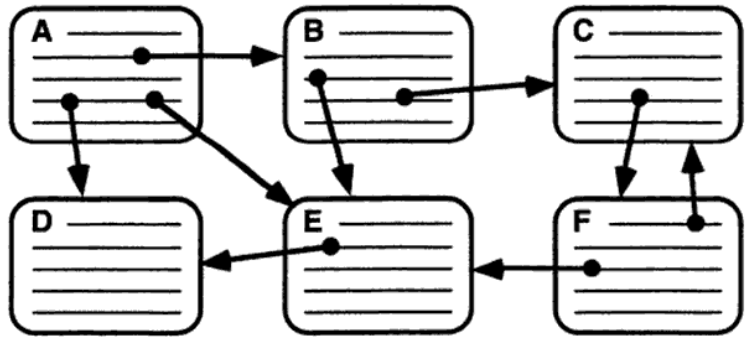
\includegraphics[width=0.8\textwidth]{image/nielsenLink}
	\caption{Vereinfachte Ansicht eines Hypertextes \cite[S.1]{Nielsen1995}}
	\label{fig:nielsenLink}
\end{figure}

Eine Verlinkung könne, wie auch Jeff Conklin 1987 beschrieben hat, einen Token in einem Dokument als Start haben und als Ziel ein anderes Dokument \cite{Conklin1987}. Wie auf Abbildung \ref{fig:imText} zusehen, zeigt der Token $xxxx$ im Dokument $A$ auf das ganze Dokument $B$. Verlinkungen können aber auch von ganzen Dokumenten auf andere Dokumente zeigen, ohne dabei einzelne Token als Start zu haben.

\begin{figure}[!ht]
	\centering
	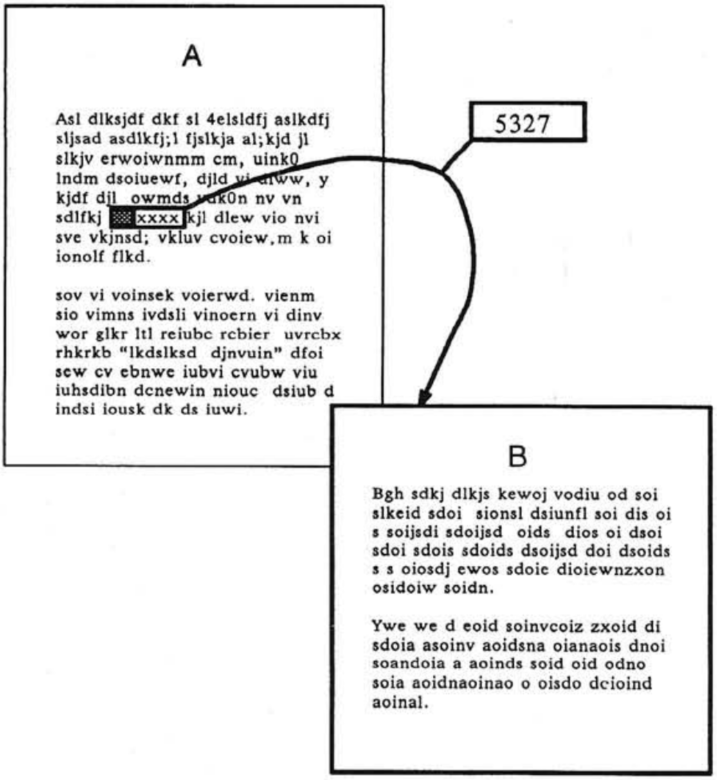
\includegraphics[width=0.8\textwidth]{image/imText}
	\caption{Ein Beispiel eines Links von in einem Text zu einem anderen Text \cite[S.34]{Conklin1987}}
	\label{fig:imText}
\end{figure}

\hl{Nodes und Edges erklaeren }\cite{Conklin1987}

Auch viel später - 1995 - beschrieb Jakob Nielsen in dem Buch Multimedia and Hpertext: The Internet and Beyond, ein Hypertext-System ganz ähnlich: \glqq The simplest way to define hypertext is to contrast it with traditional text like a book. All traditional text, whether in printed form or in computer files, is sequential, meaning that there is a single linear sequence defining the order in which the text is to be read. [...] Hypertext is nonsequential; there is no single order that determines the sequence in which the text is to be read. [...]\grqq{ }\cite[S.1]{Nielsen1995}. Er beschrieb allerdings ein Hypertext-System als gänzlich ohne sequentielle Reihenfolge. Buchs \glqq trails\grqq{ }würden durch sogenannte \glqq trail blazers\grqq{ }erstellt\cite[S.35]{Nielsen1995}.

\end{section}
